\chapter{Geração aleatória de \emph{$k$-trees}}
\label{cap:geracao}

O problema de gerar \emph{$k$-trees} está intimamente relacionado ao problema de codificá-las e decodificá-las. De fato, se há uma codificação bijetiva que associa \emph{$k$-trees} a \emph{strings}, basta gerar \emph{strings} aleatórias para gerar \emph{$k$-trees} aleatórias.

Neste capítulo, apresentamos o problema de codificar \emph{$k$-trees}, discutimos a solução linear para codificar e decodificar \emph{$k$-trees} de forma bijetiva proposta por Caminiti et al. \cite{caminiti}, explicamos como ela foi implementada neste trabalho para gerar \emph{$k$-trees} aleatórias e mostramos os resultados obtidos.

\section{Codificando árvores e \emph{$k$-trees}}

O problema de codificar árvores já foi amplamente estudado na literatura. Como destaca Caminiti et al. \cite{caminiti}:

\begin{quotation}
  Codificar árvores rotuladas por meio de \emph{strings} de rótulos de vértices é uma alternativa interessante à representação usual de estruturas de dados de árvore na memória e tem muitas aplicações práticas (por exemplo, algoritmos evolucionários sobre árvores, geração aleatória de árvores, compressão de dados e computação do volume de floresta de grafos). Diversos códigos bijetivos diferentes que realizam associações entre árvores rotuladas e \emph{strings} de rótulos foram introduzidas. De um ponto de vista algorítmico, o problema foi cuidadosamente investigado e algoritmos ótimos de codificação e decodificação desses códigos são conhecidos.
\end{quotation}

Em 1889, Cayley \cite{cayley} demonstrou que para um conjunto de $n$ vértices distintos existem $n^{n-2}$ árvores possíveis. Desde lá, foram criados vários códigos para associar \emph{strings} e árvores.

Um dos mais conhecidos é o código de Prüfer \cite{prufer}, que surgiu em 1918 e é bijetivo, associando cada árvore (rotulada) de $n$ vértices a uma lista distinta de comprimento $n-2$ no alfabeto dos rótulos da árvore.

Codificar uma árvore usando o código de Prüfer é trivial: basta remover iterativamente as folhas da árvore até que apenas dois vértices sobrem, escolhendo sempre a folha de memor rótulo. Quando uma folha é removida, adiciona-se ao código o rótulo do seu vizinho.

A figura \ref{fig:prufer} exemplifica a codificação de Prüfer mostrando uma árvore cujo o código resultante do algoritmo é $\{4, 4, 4, 5\}$.

\begin{figure}
  \centering
  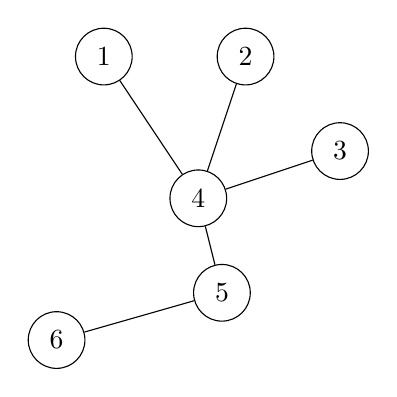
\begin{tikzpicture}
      [scale=.6,auto=left,every node/.style={draw, circle, inner sep = 0pt, minimum width = 0.72cm}]
    \node (n1) at (1,8) {1};
    \node (n2) at (4,8) {2};
    \node (n3) at (6,6) {3};
    \node (n4) at (3,5) {4};
    \node (n5) at (3.5,3) {5};
    \node (n6) at (0,2) {6};

    \foreach \from/\to in {n1/n4, n2/n4, n3/n4, n4/n5, n5/n6}
      \draw (\from) edge (\to);
  \end{tikzpicture}

  \caption{A árvore rotulada equivalente ao código de Prüfer $\{4, 4, 4, 5\}$.}
  \label{fig:prufer}
\end{figure}

\vspace{2em}

\emph{$k$-trees} \cite{harary} são consideradas uma generalização de árvores. Há interesse considerável em desenvolver ferramentas eficientes para manipular essa classe de grafos, porque todo grafo com \emph{treewidth} $k$ é um subgrafo de uma \emph{$k$-tree} e muitos problemas NP-completos podem ser resolvidos em tempo polinomial quando restritos a grafos com \emph{treewidth} limitada, como destacado na \textbf{Introdução} deste trabalho.

Há estudos sobre a codificação de \emph{$k$-trees} há pelo menos quatro décadas. Em 1970, Rényi e Renýi apresentaram uma codificação redundante (ou seja, não bijetiva) para um subconjunto de \emph{$k$-trees} rotuladas que chamamos de \emph{$k$-trees} de Rényi e que são definidas como segue:

\begin{definition}[\emph{$k$-tree} de Rényi]
  \cite{renyi} Uma \emph{$k$-tree} de Rényi $R_k$ é uma \emph{$k$-tree} enraizada com $n$ vértices rotulados em $[1, n]$ e raiz $R = \{n-k+1, n-k+2, \cdots, n\}$.
\end{definition}

Entretanto, até onde sabemos, apenas em 2008 surgiu um código bijetivo para \emph{$k$-trees} com algoritmos lineares de codificação e decodificação. Foram esses algoritmos, propostos por Caminiti et al. \cite{caminiti}, que implementamos neste trabalho.

\section{A solução de Caminiti et al.}

O artigo \emph{``Bijective Linear Time Coding and Decoding for $k$-Trees''} \cite{caminiti} apresenta um código bijetivo para \emph{$k$-trees} rotuladas, juntamente a algoritmos lineares para realizar a codificação e a decodificação.

O código é formado por uma permutação de tamanho $k$ e uma generalização do \emph{Dandelion Code} \cite{egecioglu}, que consiste em $n-k-2$ pares (onde $n$ é o número de vértices) definidos no conjunto $\{ ( 0, \varepsilon ) \} \cup ([1,n-k] \times [1,k])$. Portanto, dizemos que a codificação das \emph{$k$-trees} associa elementos em $\mathcal{T}^n_k$ (conjunto das \emph{$k$-trees} com $n$ vértices) com elementos em:

$$
\mathcal{A}^n_k = { [1,n] \choose k } \times (\{ ( 0, \varepsilon ) \} \cup ([1,n-k] \times [1,k]))^{n-k-2}
$$

Os algoritmos consistem em uma série de transformações. Para compreendê-los, é necessário definir esqueleto de uma \emph{$k$-tree} enraizada e árvore característica:

\begin{definition}[esqueleto de uma \emph{$k$-tree} enraizada]
  \label{def:skeleton}
  \cite{caminiti} O esqueleto de uma \emph{$k$-tree} enraizada $T_k$ com raiz $R$, denotado por $S(T_k, R)$, é definido da seguinte forma recursiva:

  \begin{enumerate}
    \item Se $T_k$ é apenas o $k$-clique $R$, seu esqueleto é uma árvore com um único vértice $R$.
    \item Dada uma \emph{$k$-tree} enraizada $T_k$ com raiz $R$, obtida por $T_k'$ enraizada em $R$ através da adição de um novo vértice $v$ conectado a um $k$-clique $K$ (ver definição \ref{def:ktree}), seu esqueleto $S(T_k, R)$ é obtido adicionando a $S(T_k', R)$ um novo vértice $X = \{v\} \cup K$ e uma nova aresta $(X, Y)$, onde $Y$ é o vértice de $S(T_k', R)$ que contém $K$ com uma distância mínima da raiz. Chamamos $Y$ de pai de $X$.
  \end{enumerate}
\end{definition}

\begin{definition}[árvore característica]
  \label{def:chartree}
  \cite{caminiti} A árvore característica $T(T_k, R)$ de uma \emph{$k$-tree} enraizada $T_k$ com raiz $R$ é obtida rotulando os vértices e arestas de $S(T_k, R)$ da seguinte forma:

  \begin{enumerate}
    \item O vértice $R$ é rotulado $0$ e cada vértice $\{v\} \cup K$ é rotulado $v$;
    \item Cada aresta do vértice $\{v\} \cup K$ ao seu pai $\{v'\} \cup K'$ é rotulada com o índice do vértice em $K'$ (visualizando-o como um conjunto ordenado) que não aparece em $K$. Quando o pai é $R$ a aresta é rotulada $\varepsilon$.
  \end{enumerate}

  Note que a existência de um único vértice em $K' \setminus K$ é garantida pela definição \ref{def:skeleton}. De fato, $v'$ precisa aparecer em $K$, caso contrário $K' = K$ e o pai de $\{v'\} \cup K'$ contém $K$. Isso contradiz o fato de que cada vértice em $S(T_k, R)$ é ligado à distância mínima da raiz.
\end{definition}

A figura \ref{fig:transformation} mostra uma \emph{$k$-tree} de Rényi com $11$ vértices, seu esqueleto e sua árvore característica. O \emph{Dandelion Code} generalizado correspondente a essa árvore é $[(0, \varepsilon), (2, 0), (8, 2), (8, 1), (1, 2), (5, 2)]$.

\begin{figure}
  \begin{minipage}{0.3\textwidth}
    \centering
    \scalebox{0.75}{
      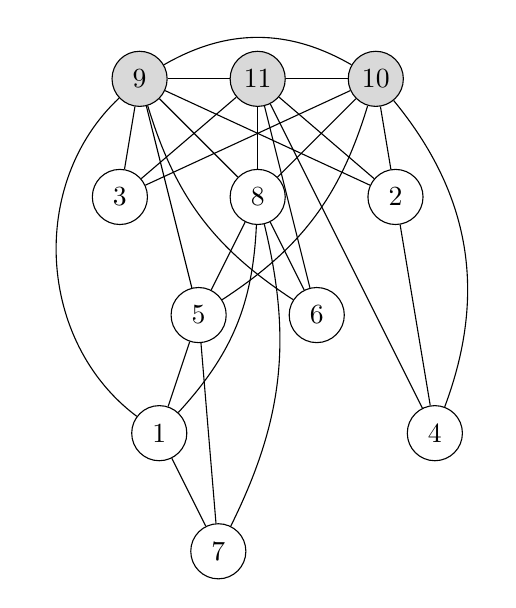
\begin{tikzpicture}
          [scale=.5,auto=left,every node/.style={draw, circle, inner sep = 0pt, minimum width = 0.7cm}]
        \node (n10) at (1,9) {3};
        \node[fill=gray!30] (n2) at (1.5,12) {9};
        \node (n1) at (2,3) {1};
        \node (n5) at (3,6) {5};
        \node (n7) at (3.5,0) {7};
        \node[fill=gray!30] (n9) at (4.5,12) {11};
        \node (n6) at (6,6) {6};
        \node (n4) at (9,3) {4};
        \node[fill=gray!30] (n3) at (7.5,12) {10};
        \node (n8) at (4.5,9) {8};
        \node (n11) at (8,9) {2};

        \foreach \from/\to in {n1/n5, n1/n7, n2/n5, n2/n8, n2/n9, n2/n10, n2/n11, n3/n8, n3/n9, n3/n10, n3/n11, n4/n9, n4/n11, n5/n7, n5/n8, n6/n8, n6/n9, n8/n9, n9/n10, n9/n11}
          \draw (\from) edge (\to);

        \draw (n1) edge [bend right=20] (n8);
        \draw (n1) edge [bend left=50] (n2);
        \draw (n2) edge [bend left] (n3);
        \draw (n2) edge [bend right=20] (n6);
        \draw (n3) edge [bend left] (n4);
        \draw (n3) edge [bend left=20] (n5);
        \draw (n7) edge [bend right=20] (n8);
      \end{tikzpicture}
    }

    (a)
  \end{minipage}\begin{minipage}{0.5\textwidth}
    \centering
    \scalebox{0.64}{\setstretch{1.0}
      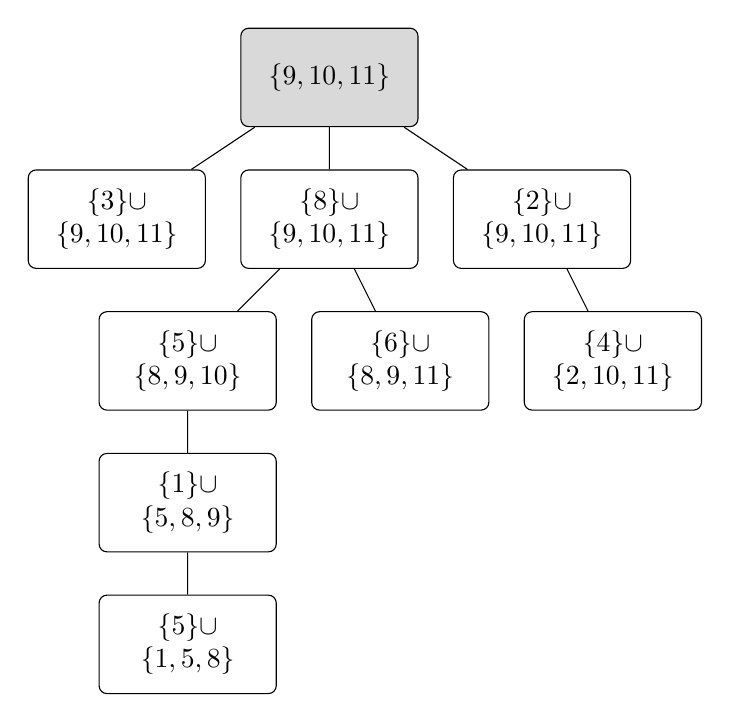
\begin{tikzpicture}
          [scale=.6,auto=left,every node/.style={draw, rectangle, rounded corners = .1cm, inner sep = 0pt, minimum height = 1.25cm, minimum width = 2.25cm, align = center}]
        \node[fill=gray!30] (n0) at (5,12) {$\{9, 10, 11\}$};
        \node (n3) at (0.5,9) {$\{3\} \cup$ \\ $\{9, 10, 11\}$};
        \node (n8) at (5,9) {$\{8\} \cup$ \\ $\{9, 10, 11\}$};
        \node (n2) at (9.5,9) {$\{2\} \cup$ \\ $\{9, 10, 11\}$};
        \node (n5) at (2,6) {$\{5\} \cup$ \\ $\{8, 9, 10\}$};
        \node (n6) at (6.5,6) {$\{6\} \cup$ \\ $\{8, 9, 11\}$};
        \node (n4) at (11,6) {$\{4\} \cup$ \\ $\{2, 10, 11\}$};
        \node (n1) at (2,3) {$\{1\} \cup$ \\ $\{5, 8, 9\}$};
        \node (n7) at (2,0) {$\{5\} \cup$ \\ $\{1, 5, 8\}$};

      \foreach \from/\to in {n0/n3, n0/n8, n0/n2, n8/n5, n8/n6, n2/n4, n5/n1, n1/n7}
        \draw (\from) edge (\to);
      \end{tikzpicture}
    }

    (b)
  \end{minipage}\begin{minipage}{0.2\textwidth}
    \centering
    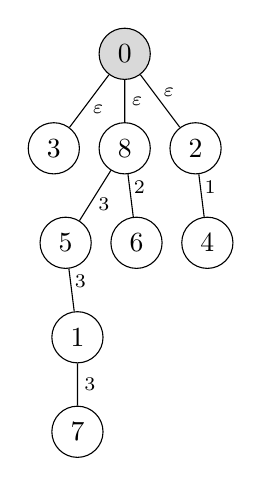
\begin{tikzpicture}
        [scale=.6,auto=left,every node/.style={draw, circle, inner sep = 0pt, minimum width = 0.65cm}]
      \node[fill=gray!30] (n0) at (5,8) {0};
      \node (n3) at (3.5,6) {3};
      \node (n8) at (5,6) {8};
      \node (n2) at (6.5,6) {2};
      \node (n5) at (3.75,4) {5};
      \node (n6) at (5.25,4) {6};
      \node (n4) at (6.75,4) {4};
      \node (n1) at (4,2) {1};
      \node (n7) at (4,0) {7};

      \foreach \from/\to/\elab in {n0/n3/$\varepsilon$, n0/n8/$\varepsilon$, n0/n2/$\varepsilon$, n8/n5/3, n8/n6/2, n2/n4/1, n5/n1/3, n1/n7/3}
        \draw (\from) -- (\to) node [draw=none, minimum width = 0.3cm, midway] {\scriptsize \elab};
    \end{tikzpicture}

    (c)
  \end{minipage}

  \caption{
    \textbf{(a)} Uma \emph{$3$-tree} de Rényi $R_3$ com 11 vértices e raiz $\{9, 10, 11\}$.
    \textbf{(b)} O esqueleto de $R_3$.
    \textbf{(c)} A árvore característica de $R_3$.
  }
  \label{fig:transformation}
\end{figure}

\subsection{Codificação}

O algoritmo para codificar uma \emph{$k$-tree} rotulada consiste em cinco passos. Aqui apresentamos esse algoritmo detalhando nossa implementação.

\begin{algorithm}[Algoritmo de codificação]
  \textbf{Entrada:} uma \emph{$k$-tree} $T_k$ com $n$ vértices\\
  \textbf{Saída:} um código em $\mathcal{A}^n_k$

  \begin{enumerate}
    \item Identificar $Q$, o $k$-clique adjacente à folha de maior rótulo $l_M$ de $T_k$;
    \item Através de um processo de re-rotulação $\phi$ (computado a partir de $Q$ e detalhado a seguir), transformar $T_k$ numa \emph{$k$-tree} de Rényi $R_k$;
    \item Gerar a árvore característica $T$ para $R_k$;
    \item Computar o \emph{Dandelion Code} generalizado $S$ para $T$;
    \item Remover da \emph{string} obtida $S$ o par correspondente a $\phi(l_M)$;
  \end{enumerate}

  O algoritmo retorna o par $(Q, S)$ computado durante esse processo.

  \vspace{2em}

  Na nossa implementação, uma \emph{$k$-tree} (estrutura definida no pacote {\tt ktree}) é representada através de uma lista de adjacências ({\tt Adj}) e um inteiro $k$ ({\tt K}). % TODO: é preciso definir lista de adjacência (em Fundamentos?).

  O algoritmo de codificação é implementado pela função {\tt CodingAlgorithm} do pacote {\tt codec}. A seguir, detalhamos os cinco passos.

  \begin{step}
    Primeiramente precisamos encontrar $l_M$, a folha de $T_k$ com maior rótulo. Uma folha em uma \emph{$k$-tree} consiste em um vértice de grau $k$, portanto basta iterar na lista de adjacências em ordem decrescente nos rótulos até encontrar um vértice com grau $k$. Isso foi implementado na função {\tt FindLm}, localizada no pacote {\tt ktree}.

    Encontrado $l_M$, atribuímos a $Q$ a lista {\tt Adj[$l_M$]} (ver função {\tt GetQ} do pacote {\tt ktree}.
  \end{step}

  \begin{step}
    Queremos transformar $T_k$ numa \emph{$k$-tree} de Rényi enraizada em $Q$. Para isso, precisamos definir uma permutação que associe os vértices de $Q$ a $\{n-k+1, n-k+2, \cdots, n\}$. A função de permutação, que chamamos de $\phi$, é definida da seguinte forma:

    \begin{enumerate}
      \item Se $q_i$ é o $i$-ésimo menor vértice em $Q$, fazemos $\phi(q_i) = n-k+i$;
      \item Para cada $q \not \in Q \cup \{n-k+1, \cdots, n\}$, fazemos $\phi(q) = q$;
      \item O restante dos valores são usados para fechar os ciclos de permutação, ou seja, para cada $q \in \{n-k+1, \cdots, n\} \setminus Q$, fazemos $\phi(q) = i$ tal que $\phi^j(i) = q$ e $j$ é maximizado.
    \end{enumerate}

    Essa computação é implementada pela função {\tt ComputePhi} no pacote {\tt ktree}.

    Usamos a função $\phi$ para re-rotular os vértices de $T_k$, obtendo a \emph{$k$-tree} de Rényi $R_k$. A implementação desse processo foi realizada na função {\tt Relabel} do pacote {\tt ktree}.

    A figura \ref{fig:phi} mostra uma representação gráfica da função $\phi$ usada para re-rotular a \emph{$3$-tree} mostrada na figura \ref{fig:rootedktree} com $Q = \{2, 3, 9\}$ produzindo a \emph{$k$-tree} de Rényi mostrada na figura \ref{fig:transformation}(a).

    \begin{figure}
      \centering
      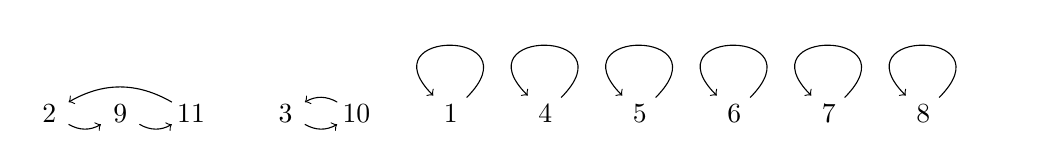
\begin{tikzpicture}
          [scale=.6,auto=left,every node/.style={circle, inner sep = 0pt, minimum width = 0.55cm}]
        \node (n2) at (1,0) {2};
        \node (n9) at (2.5,0) {9};
        \node (n11) at (4,0) {11};

        \node (n3) at (6,0) {3};
        \node (n10) at (7.5,0) {10};

        \node (n1) at (9.5,0) {1};

        \node (n4) at (11.5,0) {4};

        \node (n5) at (13.5,0) {5};

        \node (n6) at (15.5,0) {6};

        \node (n7) at (17.5,0) {7};

        \node (n8) at (19.5,0) {8};

        \foreach \from/\to in {n2/n9, n9/n11, n11/n2, n3/n10, n10/n3}
          \draw (\from) edge[->,bend right] (\to);

        \foreach \vv in {n1, n4, n5, n6, n7, n8}
          \draw (\vv) edge[loop] (\vv);
      \end{tikzpicture}
      % TODO: melhorar desenho

      \caption{Representação gráfica da função $\phi$ computada para a \emph{$3$-tree} mostrada na figura \ref{fig:rootedktree}.}
      \label{fig:phi}
    \end{figure}
  \end{step}

  \begin{step}
    As definições \ref{def:skeleton} e \ref{def:chartree} sugerem algoritmos triviais para gerar a árvore característica $T$ para a \emph{$k$-tree} de Rényi $R_k$ obtida no passo anterior por meio do seu esqueleto (o processo visto na figura \ref{fig:transformation}).

    Para garantir tempo linear, no entanto, o artigo de Caminiti et. al \cite{caminiti} sugere evitar a construção explícita do esqueleto $S(R_k)$ e construir os conjuntos de vértices e arestas de $T$ separadamente.

    Para computar o conjunto de vértices, identifica-se cliques maximais em $R_k$ através da poda sucessiva das $k$-folhas de $R_k$. Esse processo pode ser visto na função {\tt pruneRk} do pacote {\tt characteristic}. Para cada vértice $v$ podado, essa função guarda uma lista $K_v \subseteq Adj(v)$ dos exatamente $k$ vértices adjacentes a $v$ que ainda não foram podados.

    Ao fim desse processo, que tem complexidade $O(nk)$, a \emph{$k$-tree} de Rényi é reduzida apenas à sua raiz $R = \{n-k+1, \cdots, n\}$.

    A partir das listas $K_i$ ($i \in V$) e da ordem em que os vértices foram podados, constrói-se o conjunto das arestas num processo de complexidade $O(nk)$ detalhado no programa 7 do artigo \cite{caminiti} cuja implementação encontra-se na função {\tt addEdges} do pacote {\tt characteristic}.
  \end{step}

  \begin{step}
    A escrever (computar o \emph{Dandelion Code} generalizado $S$ para $T$) % TODO
  \end{step}

  \begin{step}
    A escrever (remover da \emph{string} obtida $S$ o par correspondente a $\phi(l_M)$) % TODO
  \end{step}

  A concluir. % TODO
\end{algorithm}

\subsection{Decodificação}

A escrever. % TODO

\section{Experimentos e resultados}

A escrever. % TODO

